\documentclass[tikz,border=20pt]{standalone}
\usetikzlibrary{calc}

\begin{document}
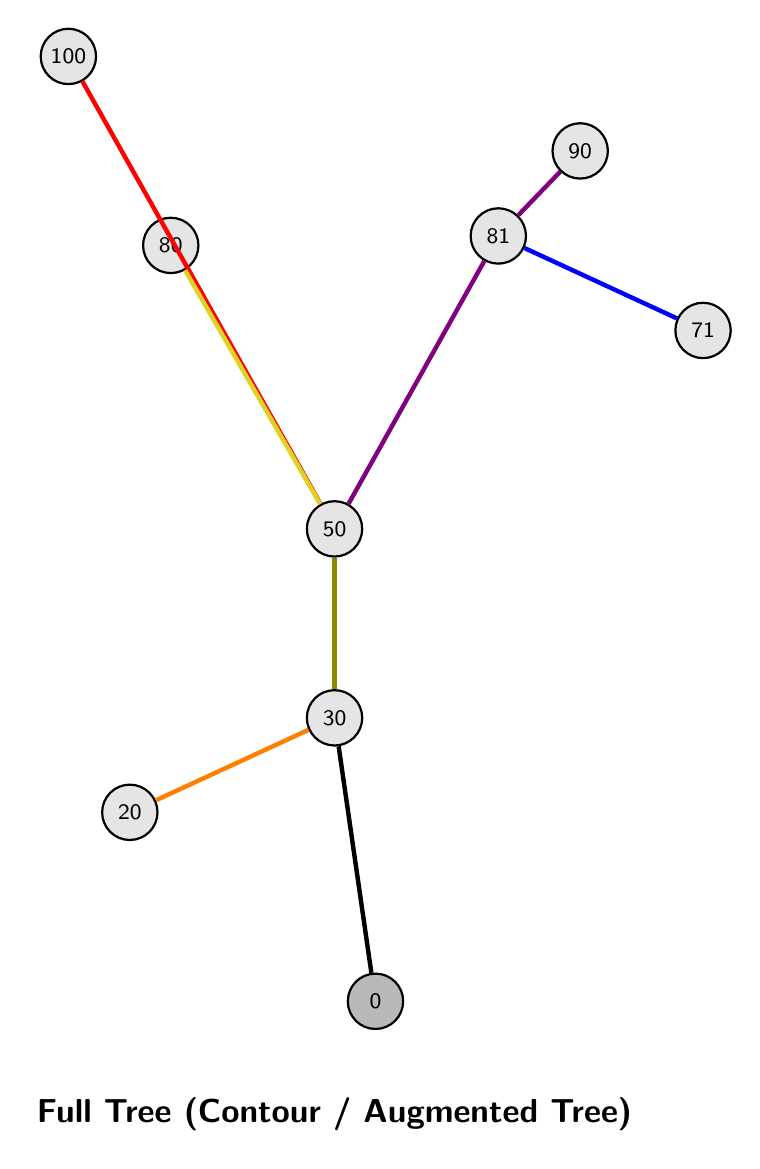
\begin{tikzpicture}[
    y=0.12cm, x=2.6cm,
    crit node/.style={circle, draw=black, fill=gray!20, thick, inner sep=1pt, minimum size=20pt, font=\sffamily\footnotesize},
    min node/.style={circle, draw=black, fill=gray!55, thick, inner sep=1pt, minimum size=20pt, font=\sffamily\footnotesize},
    reg node/.style={circle, draw=black, fill=white, inner sep=0.5pt, minimum size=14pt, font=\sffamily\tiny},
    main edge/.style={ultra thick}
]

% 临界点 (极大值、极小值、鞍点) —— 即 Contour / Augmented Tree
\node[crit node] (C100) at (-0.3, 100) {100};
\node[crit node] (C90)  at ( 2.2,  90) {90};
\node[crit node] (C81)  at ( 1.8,  81) {81};
\node[crit node] (C80)  at ( 0.2,  80) {80};
\node[crit node] (C71)  at ( 2.8,  71) {71};
\node[crit node] (C50)  at ( 1.0,  50) {50};
\node[crit node] (C30)  at ( 1.0,  30) {30};
\node[crit node] (C20)  at ( 0.0,  20) {20};
\node[min  node] (C0)   at ( 1.2,   0) {0};

% 彩色连线 (对应图中各分支颜色)
\draw[main edge, red]            (C50)  -- (C100);
\draw[main edge, yellow!85!black](C50)  -- (C80);
\draw[main edge, violet]         (C50)  -- (C81);
\draw[main edge, violet]         (C81)  -- (C90);
\draw[main edge, blue]           (C81)  -- (C71);
\draw[main edge, olive]          (C50)  -- (C30);
\draw[main edge, orange]         (C30)  -- (C20);
\draw[main edge, black]          (C30)  -- (C0);

\node[font=\sffamily\bfseries\large] at (1, -12) {Full Tree (Contour / Augmented Tree)};

\end{tikzpicture}
\end{document}
